
\section{Trägheitsmoment}


\begin{boxleft}\bla{Allgemein}
\des[\kilo\gram\per\meter\tothe{3}]{\rho}{Dichte}\\
\des[\kilo\gram\meter\tothe{2}]{J}{Massenträgheitsmoment}
\end{boxleft}\begin{boxrightshaded}
\begin{align*}
J&=\sum m_i r_i^2\\
J&=\int_m r^2 \diff m \\
J&=\int_z\int_\varphi\int_r r^3\rho \diff r \diff \varphi \diff z 
\end{align*}
\end{boxrightshaded}

\begin{boxleft}\bla{Satz von Steiner}
\des[\kilo\gram\meter\tothe{2}]{J_s}{Mtm am der alten Achse}\\
\des[\kilo\gram\meter\tothe{2}]{J_x}{Mtm am der neuen Achse $(J_x\parallel J_s)$)}\\
\des[\meter]{r}{Abstand alter und neuer Achse}
\end{boxleft}\begin{boxrightshaded}
\begin{align*}
J_x&=mr^2+J_s
\end{align*}
\end{boxrightshaded}

\begin{boxleft}\bla{Trägheitsmoment Kugel}
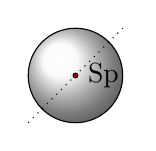
\begin{tikzpicture}[scale=.3]
  \draw[ball color=gray!5] (2,2) circle (2);
  \draw[fill=red] (2,2) circle (.1);
  \draw[dotted](0,0)--(4,4);
  \draw(2,2)node[right=1pt]{Sp};
\end{tikzpicture}\end{boxleft}\begin{boxrightshaded}
\begin{align*}
J_\text{Sp}&=\frac{2}{5}mr^2
\end{align*}
\end{boxrightshaded}

\begin{boxleft}\bla{Trägheitsmoment Zylinder}
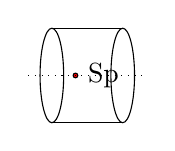
\begin{tikzpicture}[scale=.3]
  \draw (1,2) ellipse (.5 and 2);
  \draw (1,4) -- (4,4);
  \draw (1,0) -- (4,0);
  \draw (4,2) ellipse (.5 and 2);
  \draw[fill=red] (2,2) circle (.1);
  \draw[dotted](0,2)--(5,2);
  \draw(2,2)node[right=1pt]{Sp};
\end{tikzpicture}\end{boxleft}\begin{boxrightshaded}
\begin{align*}
J_\text{Sp}&=\frac{1}{2}mr^2
\end{align*}
\end{boxrightshaded}

\begin{boxleft}\bla{Trägheitsmoment Kreisring}
\end{boxleft}\begin{boxrightshaded}
\begin{align*}
J_\text{Sp}&=mr^2
\end{align*}
\end{boxrightshaded}

\begin{boxleft}\bla{Trägheitsmoment Stab}
\end{boxleft}\begin{boxrightshaded}
\begin{align*}
J_\text{Sp}=\frac{1}{12}ml^2
\end{align*}
\end{boxrightshaded}
